\documentclass[main.tex]{subfiles}
\begin{document}\newpage
\setdoublesep{0.35700 em}  % 'Bond Spacing'
\setatomsep{1.78500 em}    % 'Fixed Length'
\setbondoffset{0.18265 em} % 'Margin Width'
\newcommand{\bondwidth}{0.06642 em} % 'Line Width'
\setbondstyle{line width = \bondwidth}

\begin{fullwidth}





%%%%%%%%%%%%HEADING
\begin{multicols}{2}
\begin{tcolorbox}[enhanced jigsaw,breakable,size=title,
colback=mybrown!05,colframe=black,fonttitle=\bfseries,
title=STUDENT INFO,pad at break=1mm, break at=15cm/0pt ]
\vspace{0.2cm}
\noindent Name: \rule{5cm}{0.4pt}Date:\rule{1cm}{0.4pt}\\
Pre-lab Done: \tikzcheckmark[scale=2,black]{no mark}\quad
\end{tcolorbox}
\end{multicols}
\hfill
\vspace{0.2cm}
\begin{center}
{\large \bfseries 
Pre-lab Questions 
\par
\Huge
Heat
\\[5pt] \par}
\vspace{0.2cm}
\end{center}
\par
\noindent
\uline{  \hfill \normalsize \hfill       }
%%%%%%%%%%%%HEADING

\begin{enumerate}
% PELAB 1
\item When ice melts is heat lost or gained? Explain.
\vspace{2cm}

\item Calculate the mass of 100mL of water. Density is 1g/mL/
\vspace{2cm}

\item What happens to the temperature of water while its boiling?
\vspace{2cm}

\item How many calories are needed to boil 100g of water? ($\text{heat}_{\text{vaporization}}$=540 cal/g )
\vspace{2cm}


\item How many calories are needed to melt 100g of ice? ($\text{heat}_{\text{fusion}}$=80 cal/g )
\vspace{2cm}


\item How many calories are needed to warm up 100g of water from 10 to 50$^\circ$C? ($\text{C}_{\text{e}}$=1 cal/g/$^\circ$C )
\vspace{2cm}


\end{enumerate}


\clearpage\mbox{}\clearpage



%%%%%%%%%%%%HEADING
\begin{multicols}{2}
\begin{tcolorbox}[enhanced jigsaw,breakable,size=title,
colback=mybrown!05,colframe=black,fonttitle=\bfseries,
title=STUDENT INFO,pad at break=1mm, break at=15cm/0pt ]
\vspace{0.2cm}
\noindent Name: \rule{5cm}{0.4pt}Date:\rule{1cm}{0.4pt}\\
Pre-lab Done: \tikzcheckmark[scale=2,black]{no mark}\quad
\end{tcolorbox}
\end{multicols}
\hfill
\vspace{0.2cm}
\begin{center}
{\large \bfseries 
Experiment
\par
\Huge
Heat
\\[5pt] \par}
\vspace{0.2cm}
\end{center}
\par
\noindent
\uline{  \hfill \normalsize \hfill       }
%%%%%%%%%%%%HEADING

\vspace{0.2cm}{\large \bfseries 1. Heating curve for water}
While heating a liquid its temperature raises up until the moment the liquid boils.
\begin{steps}
    \newstep[] Place a 250mL beaker (or a 400mL) on top of a hot plate. Place a thermometer in the beaker so that it does not touch the walls of the beaker and secure it with a clam.
    \newstep[] Use a cylinder and place 100mL cool of water into the beaker.
    \newstep[] Using the thermometer record and write down the initial temperature of water.
    \newstep[] Start heating the liquid at maximum.
    \newstep[] Record the temperature in the table below every minute (you might need to add extra space in the table to accommodate all numbers). Use a stopwatch to measure time.
    \newstep[] When bubbles start appearing the liquid will be boiling. After that point record the temperature for only 5 minutes.
    \newstep[] Turn off the hop plate when the experiment is done.
        \newstep[] Plot the heating curve of water by graphing temperature (Vertical axis) vs. time (Horizontal axis).

\end{steps}




\begin{center}\begin{tabular}{ p{5cm}p{5cm}p{5cm}  }
\hline
{\linespread{1.0}\begin{center}
Time (min)\hspace{.3cm}Temperature ($^\circ$C)\\
\rule{2.0cm}{0.4pt}\hspace{.5cm}\rule{2.0cm}{0.4pt}\\
\rule{2.0cm}{0.4pt}\hspace{.5cm}\rule{2.0cm}{0.4pt}\\
\rule{2.0cm}{0.4pt}\hspace{.5cm}\rule{2.0cm}{0.4pt}\\
\rule{2.0cm}{0.4pt}\hspace{.5cm}\rule{2.0cm}{0.4pt}\\
\rule{2.0cm}{0.4pt}\hspace{.5cm}\rule{2.0cm}{0.4pt}\\
\rule{2.0cm}{0.4pt}\hspace{.5cm}\rule{2.0cm}{0.4pt}\\
\rule{2.0cm}{0.4pt}\hspace{.5cm}\rule{2.0cm}{0.4pt}\\
\rule{2.0cm}{0.4pt}\hspace{.5cm}\rule{2.0cm}{0.4pt}\\
\rule{2.0cm}{0.4pt}\hspace{.5cm}\rule{2.0cm}{0.4pt}\\
\rule{2.0cm}{0.4pt}\hspace{.5cm}\rule{2.0cm}{0.4pt}\\
\rule{2.0cm}{0.4pt}\hspace{.5cm}\rule{2.0cm}{0.4pt}\\
\rule{2.0cm}{0.4pt}\hspace{.5cm}\rule{2.0cm}{0.4pt}\\
\rule{2.0cm}{0.4pt}\hspace{.5cm}\rule{2.0cm}{0.4pt}\\
\end{center}}&    {\linespread{1.0}\begin{center}\rule{2.0cm}{0.4pt}\hspace{.5cm}\rule{2.0cm}{0.4pt}\\\rule{2.0cm}{0.4pt}\hspace{.5cm}\rule{2.0cm}{0.4pt}\\\rule{2.0cm}{0.4pt}\hspace{.5cm}\rule{2.0cm}{0.4pt}\\\rule{2.0cm}{0.4pt}\hspace{.5cm}\rule{2.0cm}{0.4pt}\\\rule{2.0cm}{0.4pt}\hspace{.5cm}\rule{2.0cm}{0.4pt}\\\rule{2.0cm}{0.4pt}\hspace{.5cm}\rule{2.0cm}{0.4pt}\\\rule{2.0cm}{0.4pt}\hspace{.5cm}\rule{2.0cm}{0.4pt}\\\rule{2.0cm}{0.4pt}\hspace{.5cm}\rule{2.0cm}{0.4pt}\\\rule{2.0cm}{0.4pt}\hspace{.5cm}\rule{2.0cm}{0.4pt}\\\rule{2.0cm}{0.4pt}\hspace{.5cm}\rule{2.0cm}{0.4pt}\\\rule{2.0cm}{0.4pt}\hspace{.5cm}\rule{2.0cm}{0.4pt}\\\rule{2.0cm}{0.4pt}\hspace{.5cm}\rule{2.0cm}{0.4pt}\\\rule{2.0cm}{0.4pt}\hspace{.5cm}\rule{2.0cm}{0.4pt}\\\rule{2.0cm}{0.4pt}\hspace{.5cm}\rule{2.0cm}{0.4pt}\\\rule{2.0cm}{0.4pt}\hspace{.5cm}\rule{2.0cm}{0.4pt}\\
\end{center}} &  {\linespread{1.0}\begin{center}\rule{2.0cm}{0.4pt}\hspace{.5cm}\rule{2.0cm}{0.4pt}\\\rule{2.0cm}{0.4pt}\hspace{.5cm}\rule{2.0cm}{0.4pt}\\\rule{2.0cm}{0.4pt}\hspace{.5cm}\rule{2.0cm}{0.4pt}\\\rule{2.0cm}{0.4pt}\hspace{.5cm}\rule{2.0cm}{0.4pt}\\\rule{2.0cm}{0.4pt}\hspace{.5cm}\rule{2.0cm}{0.4pt}\\\rule{2.0cm}{0.4pt}\hspace{.5cm}\rule{2.0cm}{0.4pt}\\\rule{2.0cm}{0.4pt}\hspace{.5cm}\rule{2.0cm}{0.4pt}\\\rule{2.0cm}{0.4pt}\hspace{.5cm}\rule{2.0cm}{0.4pt}\\\rule{2.0cm}{0.4pt}\hspace{.5cm}\rule{2.0cm}{0.4pt}\\\rule{2.0cm}{0.4pt}\hspace{.5cm}\rule{2.0cm}{0.4pt}\\\rule{2.0cm}{0.4pt}\hspace{.5cm}\rule{2.0cm}{0.4pt}\\\rule{2.0cm}{0.4pt}\hspace{.5cm}\rule{2.0cm}{0.4pt}\\\rule{2.0cm}{0.4pt}\hspace{.5cm}\rule{2.0cm}{0.4pt}\\\rule{2.0cm}{0.4pt}\hspace{.5cm}\rule{2.0cm}{0.4pt}\\\rule{2.0cm}{0.4pt}\hspace{.5cm}\rule{2.0cm}{0.4pt}\\
\end{center}}                 \\
\hline\end{tabular}\end{center}
 

\end{fullwidth}




\newpage
\begin{fullwidth}
\begin{center}
 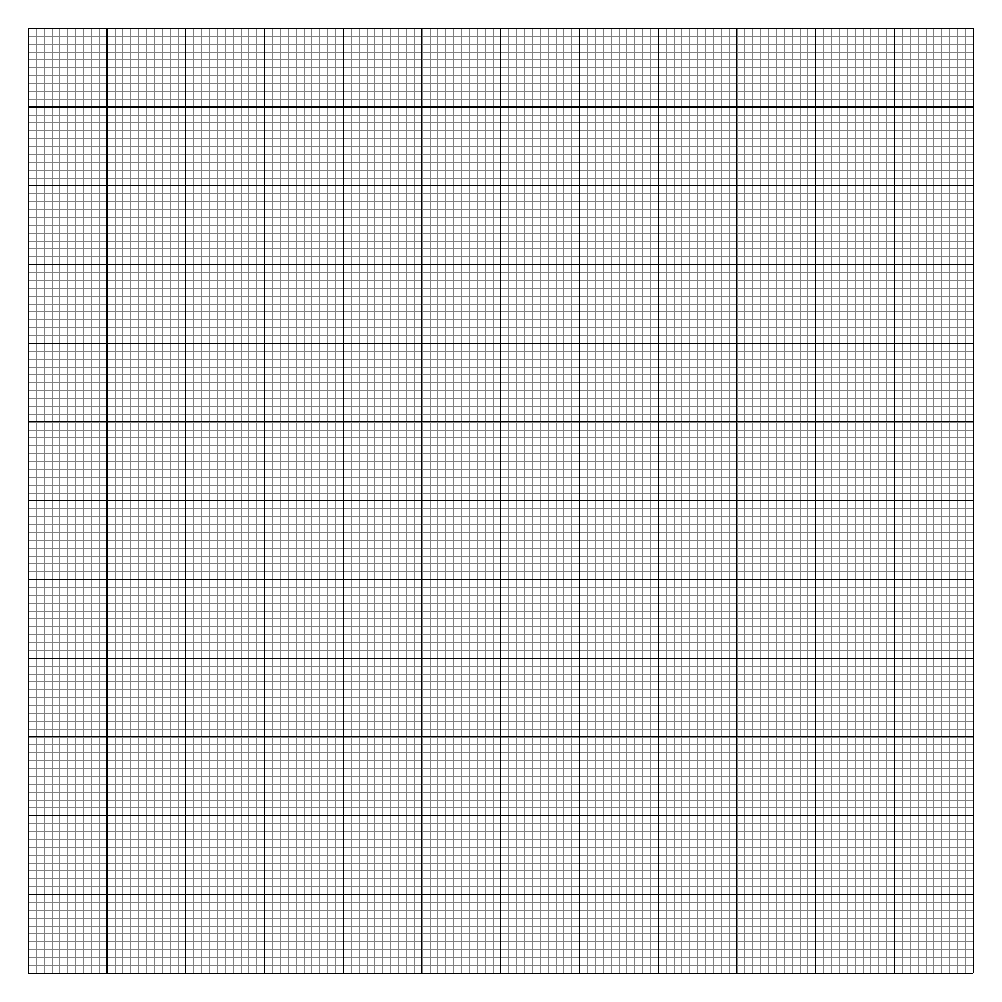
\begin{tikzpicture}
 \draw[step=1mm,help lines] (0,0) grid (120mm,120mm);
 \draw[step=10mm] (0,0) grid (120mm,120mm);
\end{tikzpicture}
\end{center}

\vspace{0.2cm}{\large \bfseries 2. Cooling curve of salol}
Phenyl salicylate, or salol, is a chemical once used in sunscreens, phenyl salicylate and now used in the manufacture of some polymers, lacquers, adhesives, waxes, and polishes. This chemical is solid at room temperature. The goal of this mini experiment is to draw the cooling curve of melted salol.
\begin{steps}
    \newstep[] Half-fill a 400mL beaker with water. Add boiling chips and start boiling the liquid with a hot plate. This is a water bath meant to melt salol.
        \newstep[]  Place the salol container in the water bath. Add a thermometer inside the salol tube to control its temperature. Melt the solid completely. Never warm up salol beyond 80$^\circ$C.
        \newstep[]  When salol is all melter stop the hot plate and start recording temperature every minute. Write down the results in the table below.
    \newstep[] After solid forms, continue measuring temperature for five more minutes.
      \newstep[] Write down the measurement in the table below. 
      \newstep[] Plot the heating curve of water by graphing temperature (Vertical axis) vs. time (Horizontal axis).
\end{steps}


\end{fullwidth}


\newpage
\begin{fullwidth}
\begin{center}\begin{tabular}{ p{5cm}p{5cm}p{5cm}  }
\hline
{\linespread{1.0}\begin{center}
Time (min)\hspace{.3cm}Temperature ($^\circ$C)\\
\rule{2.0cm}{0.4pt}\hspace{.5cm}\rule{2.0cm}{0.4pt}\\
\rule{2.0cm}{0.4pt}\hspace{.5cm}\rule{2.0cm}{0.4pt}\\
\rule{2.0cm}{0.4pt}\hspace{.5cm}\rule{2.0cm}{0.4pt}\\
\rule{2.0cm}{0.4pt}\hspace{.5cm}\rule{2.0cm}{0.4pt}\\
\rule{2.0cm}{0.4pt}\hspace{.5cm}\rule{2.0cm}{0.4pt}\\
\rule{2.0cm}{0.4pt}\hspace{.5cm}\rule{2.0cm}{0.4pt}\\
\rule{2.0cm}{0.4pt}\hspace{.5cm}\rule{2.0cm}{0.4pt}\\
\rule{2.0cm}{0.4pt}\hspace{.5cm}\rule{2.0cm}{0.4pt}\\
\rule{2.0cm}{0.4pt}\hspace{.5cm}\rule{2.0cm}{0.4pt}\\
\rule{2.0cm}{0.4pt}\hspace{.5cm}\rule{2.0cm}{0.4pt}\\
\rule{2.0cm}{0.4pt}\hspace{.5cm}\rule{2.0cm}{0.4pt}\\
\rule{2.0cm}{0.4pt}\hspace{.5cm}\rule{2.0cm}{0.4pt}\\
\rule{2.0cm}{0.4pt}\hspace{.5cm}\rule{2.0cm}{0.4pt}\\
\end{center}}&    {\linespread{1.0}\begin{center}\rule{2.0cm}{0.4pt}\hspace{.5cm}\rule{2.0cm}{0.4pt}\\\rule{2.0cm}{0.4pt}\hspace{.5cm}\rule{2.0cm}{0.4pt}\\\rule{2.0cm}{0.4pt}\hspace{.5cm}\rule{2.0cm}{0.4pt}\\\rule{2.0cm}{0.4pt}\hspace{.5cm}\rule{2.0cm}{0.4pt}\\\rule{2.0cm}{0.4pt}\hspace{.5cm}\rule{2.0cm}{0.4pt}\\\rule{2.0cm}{0.4pt}\hspace{.5cm}\rule{2.0cm}{0.4pt}\\\rule{2.0cm}{0.4pt}\hspace{.5cm}\rule{2.0cm}{0.4pt}\\\rule{2.0cm}{0.4pt}\hspace{.5cm}\rule{2.0cm}{0.4pt}\\\rule{2.0cm}{0.4pt}\hspace{.5cm}\rule{2.0cm}{0.4pt}\\\rule{2.0cm}{0.4pt}\hspace{.5cm}\rule{2.0cm}{0.4pt}\\\rule{2.0cm}{0.4pt}\hspace{.5cm}\rule{2.0cm}{0.4pt}\\\rule{2.0cm}{0.4pt}\hspace{.5cm}\rule{2.0cm}{0.4pt}\\\rule{2.0cm}{0.4pt}\hspace{.5cm}\rule{2.0cm}{0.4pt}\\\rule{2.0cm}{0.4pt}\hspace{.5cm}\rule{2.0cm}{0.4pt}\\\rule{2.0cm}{0.4pt}\hspace{.5cm}\rule{2.0cm}{0.4pt}\\
\end{center}} &  {\linespread{1.0}\begin{center}\rule{2.0cm}{0.4pt}\hspace{.5cm}\rule{2.0cm}{0.4pt}\\\rule{2.0cm}{0.4pt}\hspace{.5cm}\rule{2.0cm}{0.4pt}\\\rule{2.0cm}{0.4pt}\hspace{.5cm}\rule{2.0cm}{0.4pt}\\\rule{2.0cm}{0.4pt}\hspace{.5cm}\rule{2.0cm}{0.4pt}\\\rule{2.0cm}{0.4pt}\hspace{.5cm}\rule{2.0cm}{0.4pt}\\\rule{2.0cm}{0.4pt}\hspace{.5cm}\rule{2.0cm}{0.4pt}\\\rule{2.0cm}{0.4pt}\hspace{.5cm}\rule{2.0cm}{0.4pt}\\\rule{2.0cm}{0.4pt}\hspace{.5cm}\rule{2.0cm}{0.4pt}\\\rule{2.0cm}{0.4pt}\hspace{.5cm}\rule{2.0cm}{0.4pt}\\\rule{2.0cm}{0.4pt}\hspace{.5cm}\rule{2.0cm}{0.4pt}\\\rule{2.0cm}{0.4pt}\hspace{.5cm}\rule{2.0cm}{0.4pt}\\\rule{2.0cm}{0.4pt}\hspace{.5cm}\rule{2.0cm}{0.4pt}\\\rule{2.0cm}{0.4pt}\hspace{.5cm}\rule{2.0cm}{0.4pt}\\\rule{2.0cm}{0.4pt}\hspace{.5cm}\rule{2.0cm}{0.4pt}\\\rule{2.0cm}{0.4pt}\hspace{.5cm}\rule{2.0cm}{0.4pt}\\
\end{center}}                 \\
\hline\end{tabular}\end{center}
\begin{center}
 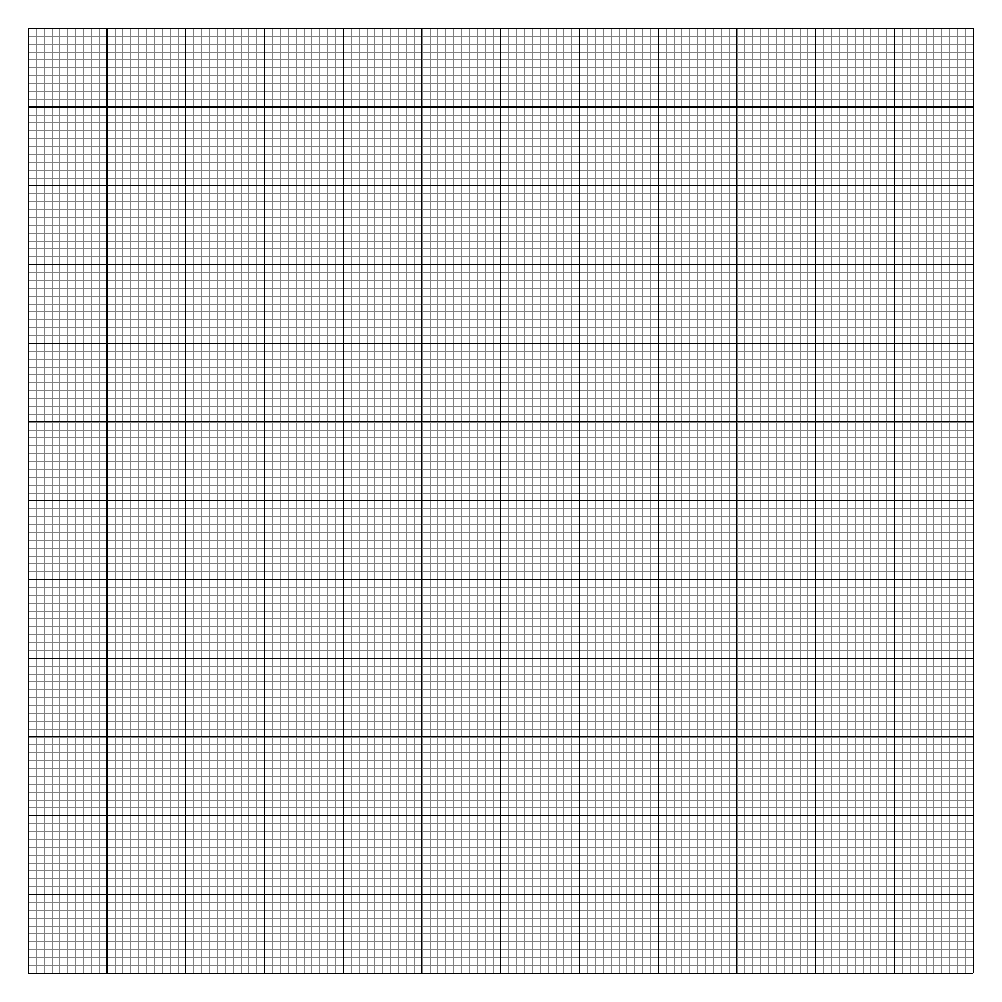
\begin{tikzpicture}
 \draw[step=1mm,help lines] (0,0) grid (120mm,120mm);
 \draw[step=10mm] (0,0) grid (120mm,120mm);
\end{tikzpicture}
\end{center}
\end{fullwidth}

\newpage
\begin{fullwidth}

\vspace{0.2cm}{\large \bfseries 3. Heat of fusion of ice}
The goal of this mini experiment is to calculate an estimate of the heat of fusion of ice. You will do this by using a calorimeter (a double styrofoam cup) and a thermometer.
\begin{steps}
    \newstep[] Weight a empty double styrofoam cup and record its mass.
 \newstep[] Add 100mL of water to the cup and weight again. Record the new mass.
  \newstep[] Record the initial temperature of water with a thermometer.
   \newstep[] Add crushed ice to the cup with water. The amount of ice should fill half of a 100mL beaker. 
    \newstep[] Close the calorimeter until all the ice is melted. Record the final temperature.
     \newstep[] Weight the cup with water and the melted ice and record the final mass.
\end{steps}


\begin{center}\begin{tabular}{ p{2.0cm}p{7.5cm}p{3cm}p{5cm}  }
\hline
 \begin{center}\mycircled{1}\end{center} &\begin{center}Mass of the calorimeter (g)\end{center}&&\begin{center}\rule{3.0cm}{0.4pt}\end{center}\\
   \begin{center}\mycircled{2}\end{center} & \begin{center}Mass of the calorimeter+ water (g)\end{center}&&\begin{center}\rule{3.0cm}{0.4pt}\end{center}\\
      \begin{center}\mycircled{2}\hspace{0.1cm}$-$\hspace{0.1cm}\mycircled{1}\end{center} & \begin{center}Mass of the water,$m_{water}$ (g)\end{center}&&\begin{center}\rule{3.0cm}{0.4pt}\end{center}\\
  \begin{center}\mycircled{3}\end{center} & \begin{center}Initial temperature of water ($^\circ$C) \end{center}&&\begin{center}\rule{3.0cm}{0.4pt}\end{center}\\
  \begin{center}\mycircled{4}\end{center}& \begin{center}Final temperature of water (when ice is melted) ($^\circ$C) \end{center}&&\begin{center}\rule{3.0cm}{0.4pt}\end{center}\\
        \begin{center}\mycircled{4}\hspace{0.1cm}$-$\hspace{0.1cm}\mycircled{3}\end{center} & \begin{center}Temperature change, $\Delta T$ ($^\circ$C)\end{center}&&\begin{center}\rule{3.0cm}{0.4pt}\end{center}\\

  \begin{center}\mycircled{5}\end{center}& \begin{center}Mass of the calorimeter+ water + melted ice (g) \end{center}&&\begin{center}\rule{3.0cm}{0.4pt}\end{center}\\
          \begin{center}\mycircled{5}\hspace{0.1cm}$-$\hspace{0.1cm}\mycircled{2}\end{center} & \begin{center}Ice mass, $m_{ice}$ (g)\end{center}&&\begin{center}\rule{3.0cm}{0.4pt}\end{center}\\


\hline\end{tabular}\end{center}


Calculate the fusion heat of ice by using the following formula, in which $C_{e, water}$ is the specific heat of water (1cal/g/$^\circ$C):
\begin{equation*}
m_{ice}\times Q_{fusion}+m_{water}\times C_{e, water}\times \Delta T=0
\end{equation*}
\hspace{2cm}
\flushright {$Q_{fusion}=$\rule{3.0cm}{0.4pt}}

\end{fullwidth}


\newpage
\begin{fullwidth}
\vspace{0.2cm}{\large \bfseries 6. PostLab questions }
\begin{enumerate}
\item Label the different areas of the heating and cooling curves you plotted with the labels: (s), (l) or (g), representing solid, liquid or gas.
\vspace{2.5cm}
\item  According to your plot, what is the boiling temperature of water. Is this value you measured reasonable? If not say why.
\vspace{2.5cm}
\item According to your plot, what is the freezing temperature of salol. 
\vspace{2.5cm}
\end{enumerate}

\end{fullwidth}

\end{document}